%% This presentation was based on Tim Osgood's
%% excellent freely available template:
%% timhosgood@gmail.com %%
%% Thank you

\documentclass{beamer}
\usepackage[utf8]{inputenc}
\usepackage{charter}
\usepackage{tikz}
\usepackage{graphicx}
\usepackage{amsmath}
\usepackage{amssymb}
\usepackage{epigraph}
\usepackage{trace}

\usepackage{listings}

%% Title slide formatting %%

\pgfdeclareimage[width=\paperwidth]{titlebackground}{images/title-slide-background.png}
\setbeamerfont{subtitle}{size=\tiny}
\setbeamertemplate{title page}{
	\begin{picture}(0,0)
		\put(-28.5,-163){%
			\pgfuseimage{titlebackground}
		}
		\put(0,-75){%
			\begin{minipage}[b][4.5cm][t]{0.5\textwidth}
				\color{black}
				\usebeamerfont{title}
				{\inserttitle\\[0.9cm]}
				\usebeamerfont{subtitle}
				{\insertauthor\par}
				{\insertinstitute\\[0.3cm]}
				{\insertdate}
			\end{minipage}
		}
	\end{picture}
}



%% General slide formatting %%

\definecolor{nhsdarkblue}{RGB}{0,48,135}

\pgfdeclareimage[width=1.4cm]{phntlogo}{images/phnt-logo.png}

\setbeamertemplate{headline}
{%
	\begin{picture}(0,0)
		\put(314,-30){%
			\pgfuseimage{phntlogo}
		}
		\put(20,-55){%
			\rule{320pt}{0.4pt}
		}
	\end{picture}
}

\setbeamertemplate{frametitle}
{%
	\begin{picture}(0,0)
		\put(-8,-10){%
			\normalsize\color{nhsdarkblue}\insertframetitle
		}
		\put(-7,-20){%
			\tiny\color{nhsdarkblue}\insertframesubtitle
		}
	\end{picture}
}

\setbeamertemplate{footline}
{%
	\begin{picture}(0,0)
		\put(20,30){%
			\rule{320pt}{0.4pt}
		}
		\put(100,14){%
			\color{nhsdarkblue}\insertshortdate
		}
		\put(160,14){%
			\color{nhsdarkblue}\insertshorttitle
		}
		\put(337,14){%
			\color{nhsdarkblue}\insertpagenumber
		}
	\end{picture}%
}



%% Information (author, title, etc.) %%

\title[Programming workshop]{Programming workshop: a very brief introduction}

\author{
	\sc{Mark Thurston}\\
    \textit{Radiology Registrar}
} 
\institute{
	\textit{Peninsula Radiology Academy}\\
    \textit{Plymouth}
}
\date[April 2018]{An introduction to automation with Python} % short date for footer



%% Content of slides %%

\begin{document}

    \begin{frame}[plain]
	    \titlepage
    \end{frame}


    \begin{frame}
	    \frametitle{Session aims}
	    \framesubtitle{By the end of this session, you will be able to:}

	    \begin{itemize}
		    \item Part 2: Practice
			    \begin{itemize}
				    \item set up a Python environment
				    \item run some pre-written example programs
				    \item Write your own simple example programs
			    \end{itemize}
	    \end{itemize}
	    \begin{itemize}
		    \item questions welcome throughout
	    \end{itemize}
    \end{frame}
    %

    \begin{frame}
	    \frametitle{Installing Python}

	    \begin{center}
	    
\includegraphics[height=4cm]{images/spam.jpg}
	    \end{center}
    \end{frame}

    \begin{frame}
	    \frametitle{Installing Python}
	    \framesubtitle{Getting up and running}

	    \begin{itemize}
		    \item Python is completely free to run on your computer without restrictions
		    \item no disadvantages to installation
			    \begin{itemize}
				    \item no privacy concerns I'm aware of
			    \end{itemize}
		    \item download link:
			    \begin{itemize}
				    \item \url{https://www.python.org/downloads/}
			    \end{itemize}
		    \item 64-bit version should run on all reasonably modern computers
			    \begin{itemize}
		    \item try the 32-bit version if unsuccessful
			    \end{itemize}
	    \end{itemize}
    \end{frame}
    %

    
    \begin{frame}
	    \frametitle{Starting the Python interpreter}
	    \framesubtitle{Getting started with the Python interpreter}

	    \begin{itemize}
		    \item Applications $\Rightarrow$ Utilities $\Rightarrow$ Terminal
		    \item type \textit{``python3''} at the \$ prompt
	    \end{itemize}
    \end{frame}
    %

\defverbatim[colored]\lstA{
	\begin{lstlisting}[language=Python,basicstyle=\ttfamily,keywordstyle=\color{red}]
# full definition
print( *objects, sep=' ', end='\n',
file=sys.stdout, flush=False)

# most useful part
print( *objects )
	\end{lstlisting}

}



    \begin{frame}
	    \frametitle{Your first program}
	    \framesubtitle{Hello world}

	    \begin{itemize}
		    \item Which function do you need?
	    \end{itemize}
	    \lstA
    \end{frame}
    %

\defverbatim[colored]\lstB{
	\begin{lstlisting}[language=Python,basicstyle=\ttfamily,keywordstyle=\color{black}]
Python 3.6.3 (default, Oct  3 2017, 21:45:48) 
[GCC 7.2.0] on linux
Type "help", "copyright", "credits" or "license" for more information.
	\end{lstlisting}

}


\defverbatim[colored]\lstC{
\begin{lstlisting}[language=Python,basicstyle=\ttfamily,keywordstyle=\color{red}]
>>> print("hello, world")	
\end{lstlisting}

}

    \begin{frame}
	    \frametitle{Your first program}
	    \framesubtitle{Hello world}

	    \begin{itemize}
		    \item open a terminal window and start the Python interpreter
		    \item hint: \textit{type ``python3''}
	    \end{itemize}
	    \lstB
	    \lstC
    \end{frame}
    %


    \begin{frame}
	    \frametitle{Editors}
	    \framesubtitle{Saving and running your first program}

	    \begin{itemize}
		    \item You have just run ``hello world'' \textit{interactively}
		    \item Now we are going to use a \textit{text editor} to save it as a program so you can run it whenever you like
		    \item Many text editors are available (beyond the scope of this short presentation)
			    \begin{itemize}
		    \item TextEdit is the basic editor included with macOS
		    \item Notepad is similar on Windows
			    \end{itemize}
	    \end{itemize}
    \end{frame}
    %



    \begin{frame}
	    \frametitle{Editors}
	    \framesubtitle{TextEdit}

	    \begin{itemize}
		    \item Finder $\Rightarrow$ Applications $\Rightarrow$ TextEdit
	    \end{itemize}
	    \begin{center}
	    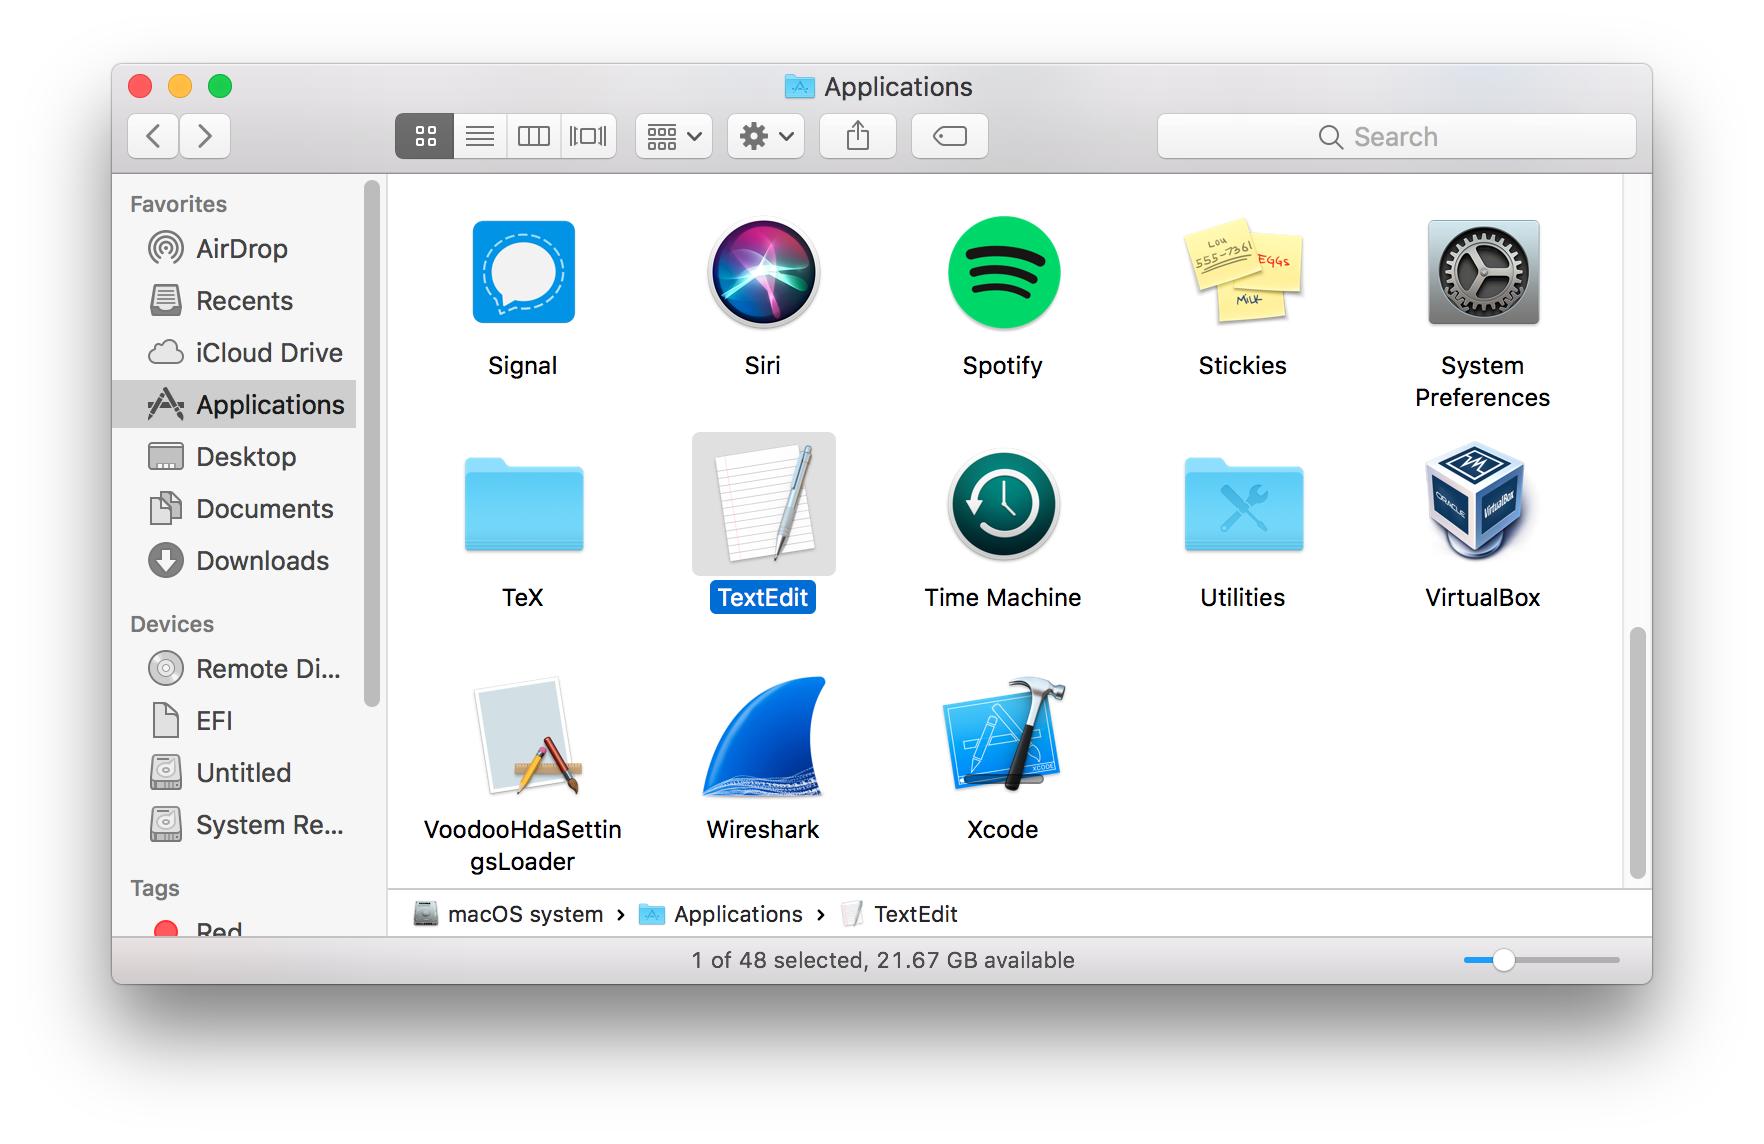
\includegraphics[height=4cm]{images/TextEdit-icon.png}
	    \end{center}
    \end{frame}
    %


    \begin{frame}
	    \frametitle{Editors}
	    \framesubtitle{TextEdit}

	    \begin{itemize}
		    \item \textit{Plain text mode} must be activated
		    \item Format $\Rightarrow$ Make plain text
	    \end{itemize}
	    \begin{center}
	    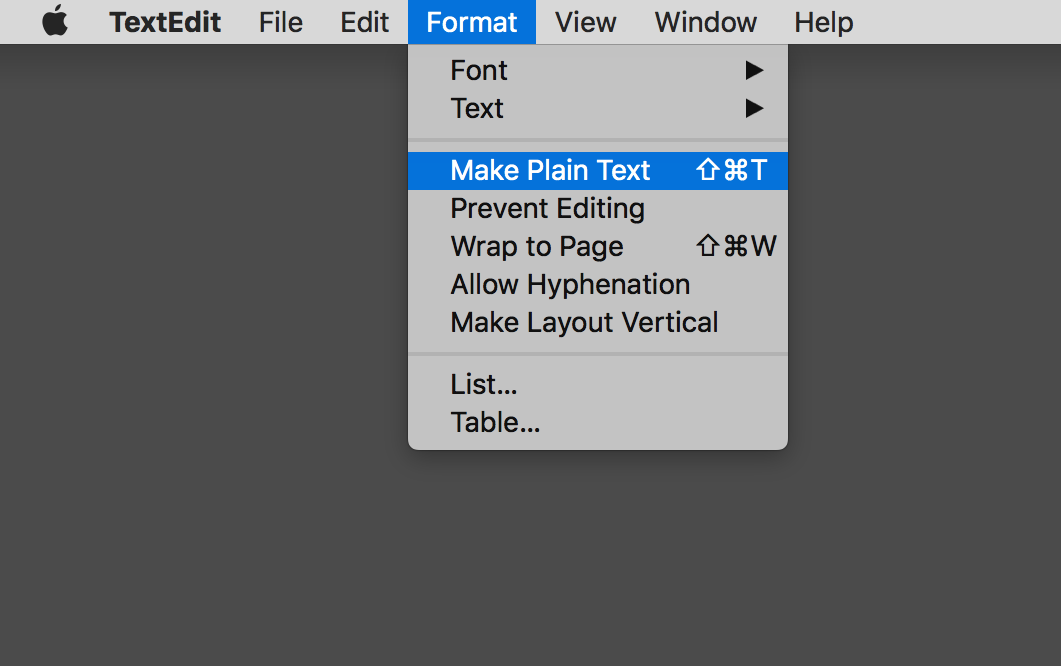
\includegraphics[height=3cm]{images/make-plain-text.png}
	    \end{center}
    \end{frame}
    %


\defverbatim[colored]\lstD{
	\begin{lstlisting}[language=Python,basicstyle=\ttfamily,keywordstyle=\color{black}]
#!/usr/bin/env python3

print("Hello world")
	\end{lstlisting}

}

    \begin{frame}
	    \frametitle{Helloworld.py}
	    \framesubtitle{Your first Python program}
	    \lstD
	    \begin{itemize}
		    \item Save the file as ``helloworld.py''
	    \end{itemize}
    \end{frame}
    %

\defverbatim[colored]\lstE{
	\begin{lstlisting}[language=Bash,basicstyle=\ttfamily,keywordstyle=\color{black}]
# you should see your program in this list
$ ls	
<file 1> <file 2> ... helloworld.py

# ensures the correct permissions to run 
$ chmod +x helloworld.py

# run your program
$ ./helloworld.py
	\end{lstlisting}

}



    \begin{frame}
	    \frametitle{Running Helloworld.py}
	    \framesubtitle{Running your first program}
	    \begin{itemize}
		    \item open a terminal window
	    \end{itemize}
	    \lstE
    \end{frame}

    
    \begin{frame}
	    \frametitle{Installing Git}
	    \framesubtitle{version control software}

	    \begin{itemize}
		    \item allows you to track changes in your source code
		    \item helpful when working on files with multiple people or in multiple places
		    \item download link:
			    \begin{itemize}
				    \item \url{https://git-scm.com/download/mac}
			    \end{itemize}
	    \end{itemize}
    \end{frame}
    %
    
\defverbatim[colored]\lstF{
	\begin{lstlisting}[language=Bash,basicstyle=\ttfamily,keywordstyle=\color{black}]
git clone https://github.com/mdvthu/Python-101
	\end{lstlisting}

}



    \begin{frame}
	    \frametitle{Clone a ``Git repo''}
	    \framesubtitle{Getting more program examples from Git}
	    
	    \begin{itemize}
		    \item more examples are available on Github:
	    \end{itemize}
	    \lstF
    \end{frame}

    \begin{frame}
	    \frametitle{Resources: books}
	    \framesubtitle{Learning resources available on the internet}
	    \begin{itemize}
		    \item Automate the boring stuff with Python: \url{https://automatetheboringstuff.com/}
		    \item Another free online tutorial: \url{https://python-textbok.readthedocs.io/en/1.0/}
	    \end{itemize}
    \end{frame}


    \begin{frame}
	    \frametitle{Resources: interactive tutorials}
	    \framesubtitle{Learning resources available on the internet}
	    \begin{itemize}
		    \item Massive open online courses: some free, some cost
			    \begin{itemize}
				    \item EdX: \url{https://www.edx.org/course?search_query=python}
				    \item Coursera: \url{https://www.coursera.org/courses?languages=en&query=python&userQuery=python}
				    \item Udacity: \url{https://eu.udacity.com/}
				    \item udemy \url{https://www.udemy.com/}
			    \end{itemize}
	    \end{itemize}
    \end{frame}

    \begin{frame}
	    \frametitle{Resources: practice to improve your skills}
	    \framesubtitle{Thousands of resources are available}
	    \begin{itemize}
		    \item coding websites
			    \begin{itemize}
				    \item \url{https://www.hackerrank.com/domains/python}
				    \item \url{https://www.codecademy.com/tracks/python}
			    \end{itemize}
		    \item open access data
			    \begin{itemize}
				    \item \url{https://data.gov.uk/}
			    \end{itemize}
		    \item read other code on \url{https://github.com}
		    \item contribute to an open source project
			    \begin{itemize}
				    \item Horos
				    \item Orthanc
				    \item OpenCV
				    \item Python
			    \end{itemize}
	    \end{itemize}
    \end{frame}


\end{document}
